%!TEX root = ../../csuthesis_main.tex
\chapter{系统总体设计}

\section{系统架构设计}

本课题期望依靠Carla仿真平台创建起一套融合了自动驾驶控制,视觉目标检测与跟踪,行为意图识别以及可视化警报功能的智能驾驶实验系统,该系统要能够针对诸如车辆,行人之类的前方交通参与者实施持续性的感知,并对其交互行为加以分析,整个系统会采取模块化的结构形式来保证各个功能部件彼此间具备较好的拓展性与独立性,从而顺应将来可能出现的算法改良和模型更替情况。

本研究所设计的系统架构如图 3-1 所示,主要包含以下六个核心模块:

\textbf{仿真环境模块(Carla Simulator):}给出高精度的虚拟城市道路,动态交通参与者,本车运动模型等仿真要素,依靠Carla给予的PythonAPI接口,该系统能够操控自动驾驶汽车在指定地图(Town10和Town01)上产生并即时行驶,给后面的感知和控制模块赋予仿真数据输入。

\textbf{本车驾驶控制模块:}通过主控脚本client\_bounding\_boxes.py中control(self,car)函数达成,其可接收仿真里关于自车的控制指令(包含加速,制动,转向等),而且具备同传感器同步,处理车辆状态之类的功能,此模块给整个系统赋予了运行的主循环以及控制接口,各个子模块都是挂在这个框架上面的。

\textbf{图像采集与传感器模块:}采用Carla中的RGB摄像头传感器并挂接到本车前部,用来收集每帧图像数据,其采集到的信息通过回调机制传递到主进程当中,接着对图像实施渲染,保存以及交给下游算法去做进一步处理,而且摄像头的设置参数(包括分辨率,视场角等)能够灵活变动,从而保证符合各类算法所规定的输入需求。

\textbf{目标检测与跟踪模块:}系统里整合了 DeepSORT 即时多目标追踪算法,每一张图片通过外部目标检测器处理之后,其检测框和类别就会被送进 DeepSORT 模型当中,依靠卡尔曼滤波和 ReID 特征关联机制来达成对目标的持续追踪,当下是以“选取最近目标”当作单目标策略,从而保证重点放在自车正前方有可能产生威胁的物体上。

\textbf{行为意图分析模块:}融合追踪目标的相对位置,速度及帧间距变动状况,采用依托物理规则的方法来执行目标行为的类别判定,此模块能够判别目标是否处于“靠近”“远离”或者“危险接近”状态,并给出语义化标签,这个功能具备轻量化特性,而且无需依靠深度模型,可以做到即时反馈与互动控制。

\textbf{结果可视化与数据存储模块:}系统凭借Pygame接口把每帧图像,边界框,跟踪ID以及行为意图标签及时渲染到显示窗口上,全部数据(图像 + 标签)每隔若干帧便会自动保存到本地目录当中,这对后续的模型训练或者分析重放很有帮助,有着不错的数据采集和重复使用能力。

\begin{figure}[H]
    \centering
    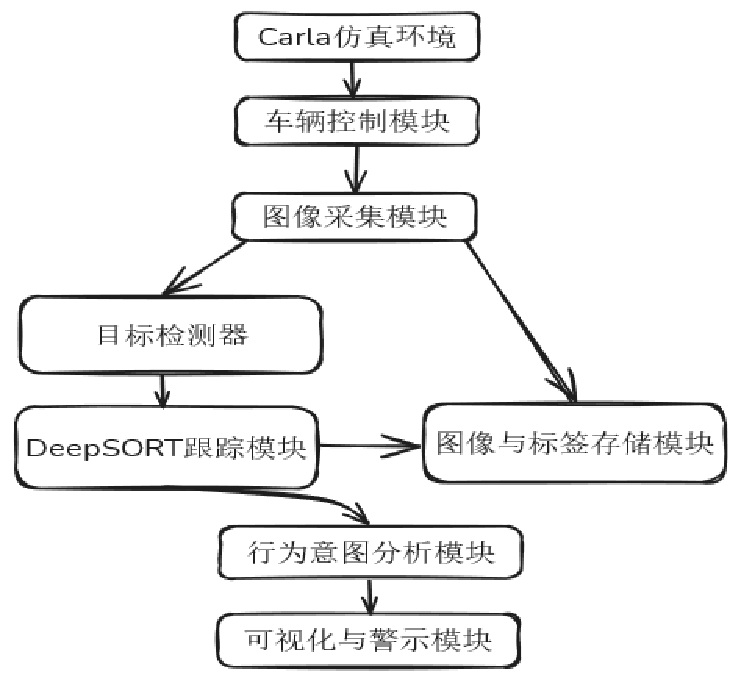
\includegraphics[width=0.8\textwidth]{images/图3 系统架构图.pdf}  % 引用转换后的 PDF 文件
    \caption{系统架构图}
    \label{fig:example_image}  % 可用于引用此图片
\end{figure}

\section{Carla 仿真平台与传感器配置}

要达成本课题里关于自动驾驶车辆的控制,视觉感知以及目标行为意图分析这些功能,系统把Carla(CarLearningtoAct)当作仿真平台来创建极为逼真的城市交通环境,Carla是IntelLabs和ComputerVisionCenter一同研发出来的一款开源自动驾驶仿真平台,它具有高保真度的城市地图,各类传感器模拟器,车辆物理引擎以及交通流经营手段,被全面用在自动驾驶研究方面。

\subsection{仿真地图选择与场景设定}

本系统选择 Carla 自带的两张典型城市地图:Town10HD 和 Town01 作为主要测试场景。

Town10HD 场景包含多车道城市道路、交通信号灯、交叉路口、障碍物遮挡、静态与动态交通参与者等复杂因素,适用于测试系统在高密度交通环境下的感知鲁棒性与行为分析准确性。

\begin{figure}[H]
    \centering
    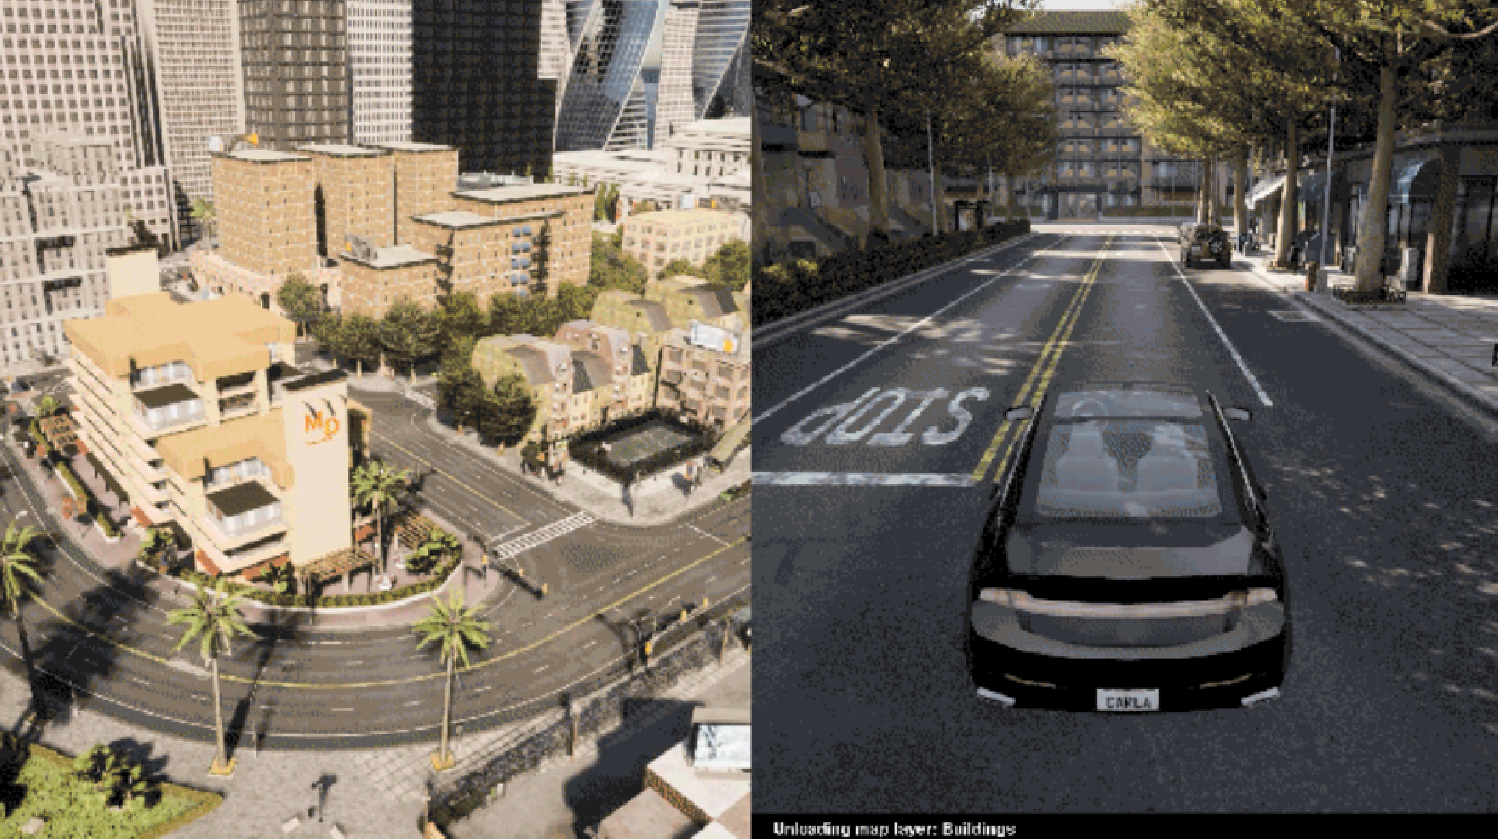
\includegraphics[width=0.8\textwidth]{images/图4 Town10HD地图展示.pdf}  % 引用转换后的 PDF 文件
    \caption{Town10HD地图展示}
    \label{fig:example_image}  % 可用于引用此图片
\end{figure}

Town01 场景则结构更为简单,适合用于算法功能验证与对比实验。

\begin{figure}[H]
    \centering
    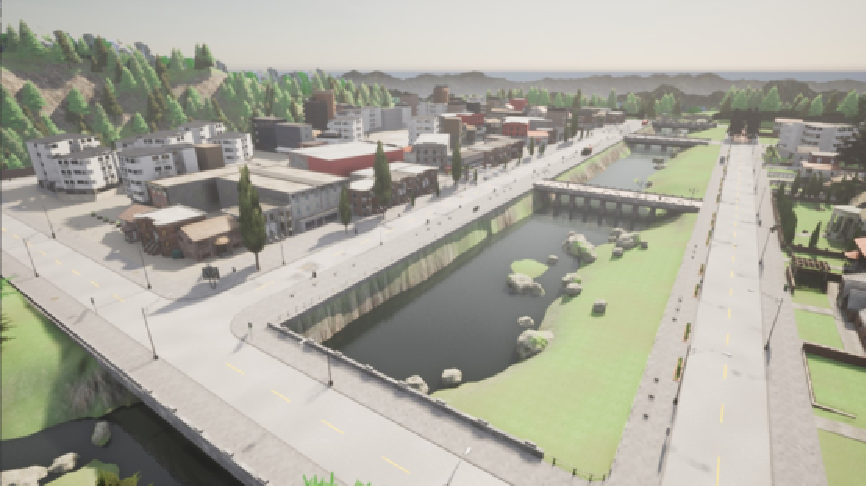
\includegraphics[width=0.8\textwidth]{images/图5 Town01地图展示.pdf}  % 引用转换后的 PDF 文件
    \caption{Town01地图展示}
    \label{fig:example_image}  % 可用于引用此图片
\end{figure}

仿真平台通过 Python API 方式加载地图并设置交通参与者生成密度与行为逻辑,确保每次启动后均可生成具有真实感的动态交通场景。

\subsection{本车模型与控制机制}

在系统初始化阶段,通过如下语句从 Carla 蓝图库中筛选车辆模型并生成本车:

\begin{figure}[H]
    \centering
    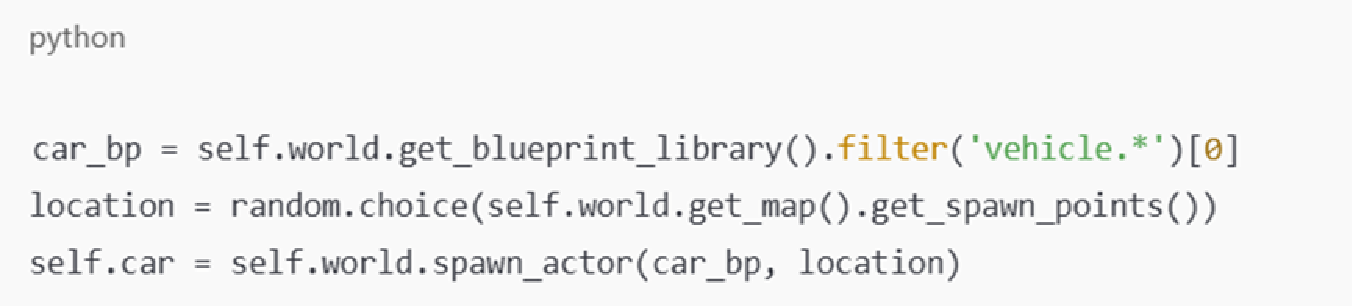
\includegraphics[width=0.8\textwidth]{images/图6 控制函数部分代码展示.pdf}  % 引用转换后的 PDF 文件
    \caption{控制函数部分代码展示}
    \label{fig:example_image}  % 可用于引用此图片
\end{figure}

车辆生成后系统对其施加控制命令,支持手动驾驶(通过键盘方向键操控)或接入后续自动控制模块。控制命令通过 Carla 的 car.apply\_control() 接口执行,包含油门、刹车、转向、手刹等基础控制量。

\subsection{摄像头传感器配置}

为获取车辆前方图像信息,系统在本车前部安装一个 RGB 摄像头传感器,其参数配置如下:

\begin{table}[htbp]
  \caption{摄像头参数配置表}
  \label{tab:camera_params}
  \centering
  \begin{tabular}{ll}
    \toprule
    参数 & 数值 \\
    \midrule
    分辨率 & 960 × 540(与系统窗口相适配) \\
    视场角(FOV) & 90° \\
    安装位置 & 自车后方5.5米,高度2.8米 \\
    俯仰角 & -15°,向下略俯视 \\
    \bottomrule
  \end{tabular}
\end{table}

摄像头配置由camera\_bp.set\_attribute()函数完成,采集的图像数据通过监听函数 self.camera.listen() 注册至主控循环,每帧图像均可进行目标检测、跟踪与意图分析,并实时渲染至用户界面或保存为数据集。

\subsection{其他配置说明}

要想让系统各个模块针对相同时间点的图像帧实施同步处理,本系统便开启Carla的同步仿真模式(synchronous\_mode=True),使得每一阶段环境状态的更新都能同传感器输出相对应,进而加强处理过程的可掌控性以及图像帧的稳定性,处于同步模式的时候,系统会按照固定频率(20FPS)去调用world.tick()以推动环境向前发展,这样就能保障传感器输出和控制行为之间存在确切的一一对应关系,有益于维持状态追踪的准确性并延续分析逻辑的连贯性。

而且,系统依靠pygame图形界面来做图像渲染工作,用numpy,cv2,json这些工具库执行图像处理,数据标注以及数据集形成方面的任务,整个系统要靠CarlaServer正常运行(直接在Windows下双击CarlaUE4.exe就能启动),从而保证模拟世界稳定又开放。

\section{项目开发环境与工具链}

为高效实现自动驾驶场景下的视觉目标跟踪与意图识别算法,并完成系统级仿真测试与可视化功能开发,本文构建了一个基于 Carla 仿真平台的完整算法开发与测试环境。本节将对本项目使用的软硬件配置、开发语言、核心依赖库与工具链进行说明。

\subsection{开发硬件平台}

实验采用配置如下表的工作站,满足实时仿真需求:

\begin{table}[htbp]
  \caption{硬件配置表}
  \label{tab:hardware_config}
  \centering
  \begin{tabular}{ll}
    \toprule
    组件 & 规格 \\
    \midrule
    CPU & Intel Core i7-10750H @ 2.60GHz \\
    GPU & NVIDIA RTX 2060 (6GB GDDR6) \\
    内存 & 16GB DDR4 \\
    存储 & 512GB NVMe SSD \\
    \bottomrule
  \end{tabular}
\end{table}

\subsection{开发软件与工具}

项目开发主要在 Windows 10 平台下进行,核心依赖环境和工具包括:

\begin{table}[htbp]
  \caption{软件工具链配置}
  \label{tab:software_stack}
  \centering
  \begin{tabular}{lll}
    \toprule
    软件 & 版本 & 用途 \\
    \midrule
    Python & 3.7.9 & 主控程序开发 \\
    Carla & 0.9.15 & 自动驾驶仿真 \\
    Pygame & 2.5.2 & 可视化界面渲染与用户交互界面 \\
    OpenCV & 4.8.0 & 图像读取与保存,数据集采集处理 \\
    deep\_sort\_realtime & 1.3.2 & 多目标跟踪 \\
    \bottomrule
  \end{tabular}
\end{table}

其中CarlaSimulator的安装与启动采用图形化模式,即双击启动CarlaUE4.exe来打开仿真服务端,而客户端代码运行时则是以TCP方式通信(默认端口2000),为保证数据同步性,系统均统一采用Carla的同步模式运行,使得传感器输出,车辆控制以及仿真时间能够严格对齐。

Python环境用Anaconda来做管理,创建单独的虚拟环境之后再通过pip install去装那些依赖库,这样就能保证版本稳定而且可重现,像deep\_sort\_realtime这种库是从PyPI上获取的,或者按照官方GitHub上的源码执行安装。





\begin{tabular}{l l}
%  \verb|\songti| & {\songti 宋体} \\
%  \verb|\heiti| & {\heiti 黑体} \\
%   \verb|\kaiti| & {\kaiti 楷体}
\end{tabular}
